\section*{Lecture 2: Set Functions}

\begin{definition}
    Let $\Cc \subseteq 2^R$ for some set $R$. We call a function $\mu:\Cc
    \xrightarrow{} \R^+_{\infty}$ \textbf{additive} if for any finite disjoint
    collection $\{E_i\}_{i=1}^n$, we have
    \begin{equation*}
        \mu(\bigcup_{i=1}^n{E_i})=\sum_{i=1}^n{\mu(E_i)}
    \end{equation*}
\end{definition}

Suppose there is an $A \in \Cc$ for which $\mu(A)$ is finite. By additivity, we
have that
\begin{equation*}
    \mu(A)=\mu(A \cup \emptyset)=\mu(A)+\mu(\emptyset)
\end{equation*}
Subtracting $\mu(A)$ from both sides of the equations then yields
\begin{equation*}
    \mu(\emptyset)=0
\end{equation*}
Moreover, if $A \subseteq B$, then notice that  $B=A \cup \com{B}{A}$, so that
\begin{equation*}
    \mu(B)=\mu(A \cup \com{B}{A})=\mu(A)+\mu(\com{B}{A})
\end{equation*}
So that
\begin{equation}
    \mu(A) \leq \mu(B)
\end{equation}
Now, in the case where $\mu(B)$ is infinite, we must also have that $\mu(A)$ is
infinite, in which case we still get the inequality.

\begin{example}\label{example_2}
    Let $R$ a set, and  $\{x_n\}$ a sequence of points of $R$. Let  $\{p_n\}$ a
    sequence of nonnegative numbers, and let $\Cc \subseteq 2^R$. Define the
    function  $\mu:\Cc \xrightarrow{} \R^+_\infty$ by $\mu(x)=\sum{p_nx_n}$
    Then $\mu$ is additive.
\end{example}

\begin{definition}
    Let $R$ a set and $\Cc \subseteq 2^R$ with $\emptyset \in \Cc$. We say that
    a function $\mu:\Cc \xrightarrow{} \R^+_\infty$ is
    \textbf{$\sigma$-additive} if for any countable disjoint collection
    $\{E_n\}$, we have
    \begin{equation*}
        \mu(\bigcup{E_n})=\sum{\mu(E_n)}
    \end{equation*}
\end{definition}

\begin{example}\label{example_3}
    Let $R=(0,1)$ and define
    \begin{equation*}
        \Cc=\{(a,b] : 0 \leq a<b<1\} \cup \{\emptyset\}
    \end{equation*}
    and define $\mu:\Cc \xrightarrow{} \R^+_\infty$ by
    \begin{equation*}
        \mu((a,b])=\begin{cases}
                    b-a, \text{ if } a=0    \\
                    \infty, \text{ if } a>0 \\
                 \end{cases}
    \end{equation*}
    Then $\mu$ is additive, but it is not  $\sigma$-additive. Let  $\{x_n\}
    \xrightarrow{} 0$ a decreasing sequence, with $x_1=\frac{1}{2}$. Then take
    \begin{equation*}
        (0,\frac{1}{2}]=\bigcup{(x_{i+1},x_i]}
    \end{equation*}
\end{example}

\begin{definition}
    Let $\Cc$ a collection of subsetes of a set $R$. We say a function $\mu:\Cc
    \xrightarrow{} \R^+_\infty$ is \textbf{continuous from below} at $E$
    provided that for any increasing seqeuence $\{E_n\}$ of subsets of $R$, we
    have $\{\mu(E_n)\} \xrightarrow{} \mu(E)$ whenever $\{E_n\} \xrightarrow{}
    E$.
\end{definition}

\begin{definition}
    Let $\Cc$ a collection of subsetes of a set $R$. We say a function $\mu:\Cc
    \xrightarrow{} \R^+_\infty$ is \textbf{continuous from above} at $E$
    provided that for any decreasing seqeuence $\{E_n\}$ of subsets of $R$, we
    have $\{\mu(E_n)\} \xrightarrow{} \mu(E)$ whenever $\{E_n\} \xrightarrow{}
    E$ and where $\mu(E_{n_0})$ if finite for some $n_0 \in \Z^+$.
\end{definition}

\begin{definition}
    Let $\Cc$ a collection of subsetes of a set $R$. We say a function $\mu:\Cc
    \xrightarrow{} \R^+_\infty$ is \textbf{continuous} at $E$ provided it is
    continuous from below at $E$, and continuous from above at $E$.
\end{definition}

\begin{lemma}\label{lemma_7}
    Let $S$ an algebra on  $R$ and  $\mu:S \xrightarrow{} \R^+_\infty$ be
    additive. Then the following are true
    \begin{enumerate}
        \item[(1)] If $\mu$ is $\sigma$-additive, then it is continuous at $E$
            for all  $E \in S$.

        \item[(2)] If $\mu$ is continuous from below, then  $\mu$ is
            $\sigma$-additive.

        \item[(3)] If $\mu$ is continuous from above at  $\emptyset$, with
            $\mu(R)$ finite, then it is $\sigma$-additive.
    \end{enumerate}
\end{lemma}
\begin{proof}
    \begin{enumerate}
        \item[(1)] Suppose that $\mu$ is sigma additive. Let  $\{E_n\}$ an
            increasing sequence of subsets of $R$ convergine to $E$.
            \begin{figure}[h]
                \centering
                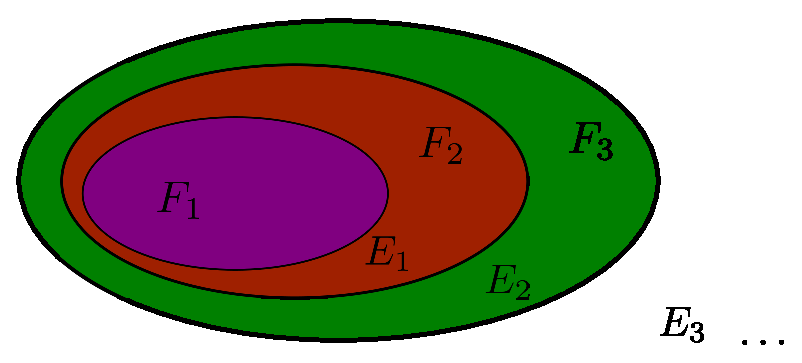
\includegraphics[scale=1]{Figures/increasing_cover.eps}
                \caption{}
                \label{figure_2}
            \end{figure}
            Let $F_1=E_1$, $F_2=\com{E_2}{E_1}$, $\dots$,
            $F_n=\com{E_n}{E_{n-1}}$, in accordance to figure \ref{figure_2}.
            Notice then that ${F_k}$ is a disjoint collection with
            $\bigcup{F_k}=\bigcup{E_n}=E$.
            Then
            \begin{equation*}
                \mu(E)=\sum{\mu(F_k)}=\lim_{n \xrightarrow{}
                \infty}{\sum_{k=1}^n{\mu(F_k)}}=\lim{\mu(F_k)}=\lim{\mu(E_n)}
            \end{equation*}
            Thus $\mu$ is continuous from below at  $E$.

            Now let $E \in S$ and let $\{E_n\}$ a decreasing sequence converging
            to $E$, and which  $\mu(E_{n_0})$ is finite for some $n_0 \in \Z^+$.
            In similar manner to what was defined for figure \ref{figure_2},
            define $G_1=\com{E_{n_0}}{E_{n_0+1}}, \dots,
            G_k=\com{E_{n_0}}{E_{n_0+k}}$. Then $\{G_k\}$ is an increasing
            sequence of disjoint subsets of $R$ with  $\{G_k\} \xrightarrow{}
            \com{E_{n_0}}{E}$. Now, since $\mu$ is  $\sigma$-additive, and
            continuous from below, we get that  $\{\mu(G_k)\} \xrightarrow{}
            \mu(\com{E_{n_0}}{E})$. So we have that
            \begin{align*}
                \mu(\com{E_{n_0}}{E}) &=  \lim{\mu(\com{E_{n_0}}{E_{n_0+k}})} \\
                                    &=  \lim{\mu(E_{n_0})}-\lim{\mu(E_{n_0+k})} \\
            \end{align*}
            then
            \begin{equation*}
                \mu(E_{n_0})-\mu(E)=\mu(E_{n_0})-\lim{\mu(E_{n_0+k})}
            \end{equation*}
            Subtracting and rearranging terms gives us the result.

        \item[(2)] Suppose that $\mu$ is continuous from below. Let
            $E=\bigcup{E_k}$ a disjoint union. Then notice that
            \begin{equation*}
                \bigcup_{k=1}^n \subseteq E
            \end{equation*}
            so that
            \begin{align*}
                \mu(\bigcup_{k=1}^n{E_k}) &\leq \mu(E), \text{ so that} \\
                \sum_{k=1}^{n}{\mu(E_k)} &\leq \mu(E), \text{ then as } n
                \xrightarrow{} \infty \\
                \sum{\mu(E_k)} &\leq \mu(E)
            \end{align*}
            Now, let $F=\bigcup_{k=1}^n{E_k} \in S$. Then $\{F_n\}
            \xrightarrow{} E$ is an increasing sequence, and since $\mu$ is
            continuous from below, we have that  $\{\mu(F_n)\} \xrightarrow{}
            \mu(E)$ so that
            \begin{equation*}
                \sum_{k=1}^n{\mu(F_k)} \xrightarrow{} \mu(E)
            \end{equation*}
            making $\mu(E) \leq \sum{\mu(E_k)}$, making $\mu$ $\sigma$-additive.

        \item[(3)] Lastly, suppose that $\mu$ is continuous from below at
            $\emptyset$, with  $\mu(R)$ finite. Let $\{E_k\}$ be an increasing
            sequence and $F_n=\bigcup_{k \geq n}{E_k}$ which defines a
            decreasing sequence $\{F_n\} \xrightarrow{} \emptyset$. By
            finiteness of $\mu(R)$, we have that $\mu(F_1)$ is also finite, and
            by continuity, that $\{m(F_n)\} \xrightarrow{} 0$. Now,
            \begin{align*}
                \mu(E) &= \mu( \bigcup_{k=1}^n{E_k} \cup \bigcup_{k \geq n}{E_k}) \\
                     &= \sum_{k=1}^n{\mu(E_k)}+\mu(F_{n+1}) \\
            \end{align*}
            Now, since $\{F_n\} \xrightarrow{} 0$, we get that
            \begin{equation*}
                \mu(E)=\sum{\mu(E_k)}
            \end{equation*}
    \end{enumerate}
\end{proof}

\begin{example}\label{example_4}
    Refering to example \ref{example_3}, we have that $\mu$ is additive, but not
     $\sigma$-additive. Take $\{E_n\} \xrightarrow{} \emptyset$ decreasign, with
     $E_n=(a_{n_1},b_{n_1}] \cup (a_{n_k},b_{n_k}]$, with $a_{n_j}<a_{n_{j+1}}$.
     If $a_{n_1}=0$, for all $n$, then we have $\mu((a_{n_1},b_{n_1}])$ is
     infinite, and there is nothing to prove. Now, if $a_{n_{k_0}}>0$ for all
     $k_0$, then $\mu$ is continuous from below at  $\emptyset$, but  $\mu$ is
     infinite.
\end{example}

\begin{theorem}\label{theorem_8}
    Let $S$ be a semialgebra on  $R$ and $\mu:S \xrightarrow{} \R^+_\infty$
    additive. Then there exists a function $\nu:Q(S) \xrightarrow{} \R^+_\infty$
    which is additive such that
    \begin{enumerate}
        \item[(1)] $\nu(A)=\mu(A)$ for all $A \in S$.

        \item[(2)] $\nu$ is unique.
    \end{enumerate}
    where $Q(S)$ is the algebra generated by $S$.
\end{theorem}
\begin{proof}
    Recall that if $A \in Q(S)$, then
    \begin{equation*}
        A=\bigcup_{k=1}^n{E_k}
    \end{equation*}
    where $\{E_k\}_{k=1}^n$ is a finite disjoint collection of elements of $S$.

    Define  $\nu:Q(S) \xrightarrow{} \R^+_\infty$ by
    \begin{equation*}
        \nu(A)=\sum{\nu(E_n)} \text{ where } \nu(E_n)=\mu(S_n) \text{ for all }
        E_n \in S
    \end{equation*}
    Let $A=\bigcup_{i=1}^m{F_i}$, then
    $\nu(A)=\sum_{i=1}^m{\mu(F_k)}=\sum_{k=1}^n{\mu(E_k)}$. Since $\mu$ is
    additive on $S$, and $E_k \subseteq S$, then
    \begin{equation*}
        E_k=E_k \cap \bigcup_{i=1}^m{F_i}=\bigcup_{i=1}^m{(E_k \cap F_i)}
    \end{equation*}
    Then
    \begin{equation*}
        \mu(E_k)=\sum{\mu(E_k \cap F_i)}
    \end{equation*}
    So that
    \begin{equation*}
        \nu(A)=\sum_{k=1}^n{\sum_{i=1}^m{\mu(E_k \cap F_i)}}
    \end{equation*}
    which makes $\sum{\mu(F_i)}=\sum{\mu(E_k)}$. Therefore $\nu$ is well
    defined.

    Now let  $A,B \in Q(S)$. Then $A=\bigcup_{i=1}^n{E_i}$ and
    $B=\bigcup_{j=1}^m{F_j}$ with $A$ and $B$ disjoint. Then we have that
    \begin{equation*}
        \nu(A \cup B)=\mu(A \cup B)=\mu(A)+\mu(B)=\nu(A)+\nu(B)
    \end{equation*}
    So that $\nu$ is additive.

    Lastly, suppose that  $\nu':Q(S) \xrightarrow{} \R^+_\infty$ is additive
    such that $\nu'(A)=\mu(A)$ for any $A \in S$. Since  $\nu(A)=\mu(A)$, take
    $B \in Q(S)$ so that $B=\bigcup_{k=1}^n{E_k}$. Then
    $\nu(B)=\sum{\nu(E_k)}=\sum{\mu(E_k)}$ and
    $\nu'(B)=\sum{\nu'(E_k)}=\sum{\mu(E_k)}$ so that $\nu(B)=\nu'(B)$ for all $B
    \in S$.
\end{proof}
\begin{corollary}
    If $\mu$ is  $\sigma$-additive, then so is  $\nu$.
\end{corollary}
